\subsection{SPIQA (LLM)}
{{\footnotesize
\noindent A workshop version of SPIQA comparing 10 LLM adapter methods on the SPIQA benchmark with scientific diagram/questions. Highlights performance differences between chain-of-thought and end-to-end adapter models.


\begin{description}[labelwidth=4cm, labelsep=1em, leftmargin=4cm, itemsep=0.1em, parsep=0em]
  \item[date:] 2024-12-13
  \item[version:] v1.0
  \item[last\_updated:] 2024-12
  \item[expired:] unknown
  \item[valid:] yes
  \item[valid\_date:] 2024-12-13
  \item[url:] \href{https://neurips.cc/virtual/2024/poster/97575}{https://neurips.cc/virtual/2024/poster/97575}
  \item[doi:] 10.48550/arXiv.2407.09413
  \item[domain:] Multimodal Scientific QA; Computer Vision
  \item[focus:] Evaluating LLMs on image-based scientific paper figure QA tasks (LLM Adapter performance)
  \item[keywords:]
    - multimodal QA
    - scientific figures
    - image+text
    - chain-of-thought prompting
  \item[licensing:] unknown
  \item[task\_types:]
    - Multimodal QA
  \item[ai\_capability\_measured:]
    - Visual reasoning
    - scientific figure understanding
  \item[metrics:]
    - Accuracy
    - F1 score
  \item[models:]
    - LLaVA
    - MiniGPT-4
    - Owl-LLM adapter variants
  \item[ml\_motif:]
    - Multimodal QA
  \item[type:] Benchmark
  \item[ml\_task:]
    - Multimodal QA
  \item[solutions:] Solution details are described in the referenced paper or repository.
  \item[notes:] Companion to SPIQA main benchmark; compares adapter strategies using same images and QA pairs.

  \item[contact.name:] Xiaoyan Zhong
  \item[contact.email:] unknown
  \item[results.links.name:] ChatGPT LLM
  \item[fair.reproducible:] Yes
  \item[fair.benchmark\_ready:] Yes
  \item[id:] spiqa\_llm
  \item[Citations:] \cite{pramanick2025spiqadatasetmultimodalquestion}
\end{description}

{\bf Ratings:} ~ \\

\begin{tabular}{p{0.15\textwidth} p{0.07\textwidth} p{0.7\textwidth}}
\hline
Rating & Value & Reason \\
\hline
dataset & 5 & Full dataset available on Hugging Face with train/test/valid splits.
 \\
documentation & 5 & Full paper available
 \\
metrics & 4 & Reports accuracy and F1; fair but no visual reasoning-specific metric.
 \\
reference\_solution & 4 & 10 LLM adapter baselines; results included without constraints.
 \\
software & 5 & Well-documented codebase available on Github
 \\
specification & 3.5 & Task of QA over scientific figures is sufficient but not fully formalized in input/output terms. No hawrdware constraints.
 \\
\hline
\end{tabular}

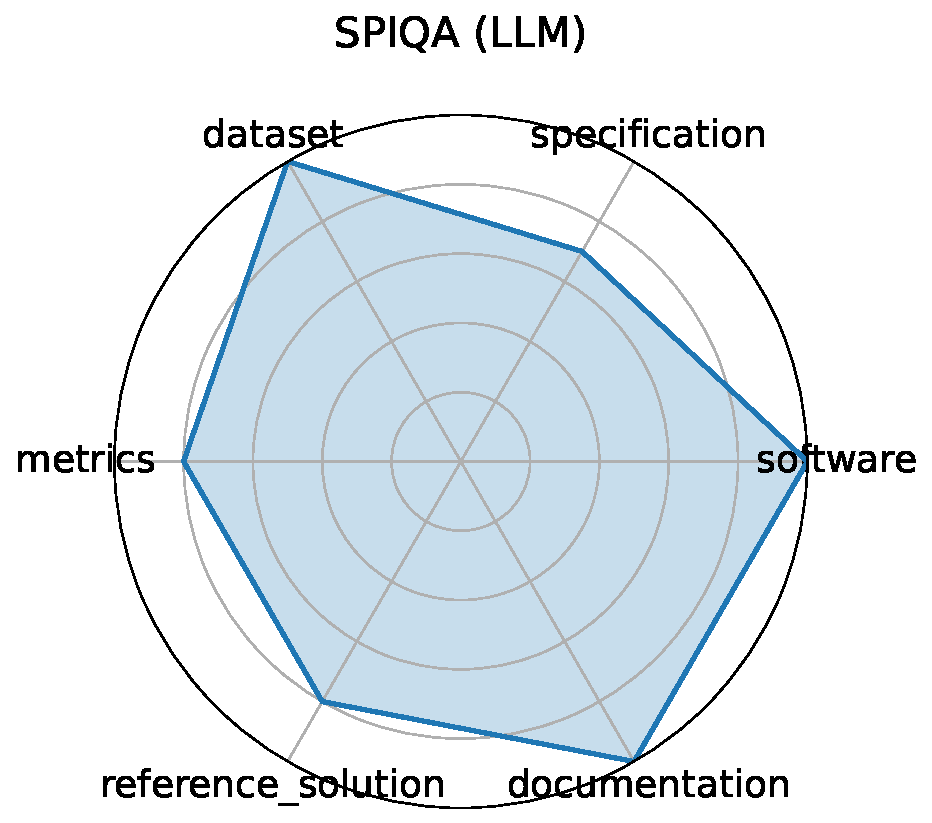
\includegraphics[width=0.2\textwidth]{spiqa_llm_radar.pdf}
}}
\clearpage